% /===========================================================================\
%
%   preamble
%
% \===========================================================================/
\documentclass{beamer}
\usetheme{Warsaw}
\usecolortheme{default}
\usefonttheme{structurebold}
\usepackage{german}
\usepackage[utf8]{inputenc}
\usepackage{graphicx} 

\usepackage{hyperref}
\usepackage{amsmath}
\usepackage{wrapfig}

% /===========================================================================\
%
%   init document
%
% \===========================================================================/

\begin{document}

% /===========================================================================\
%
%   title
%
% \===========================================================================/

\title{Deanonymisierung von Tor-Nutzern durch Ultraschall-Tracking}

\subtitle{Im Orginal: "`Talking Behind Your Back
On the Privacy \& Security of the Ultrasound Tracking Ecosystem"' von Vasilios Mavroudis und Federico Maggi}

\author{
{\rm Alexander Lüdke} (548965) \\
\and % seperate authors
{\rm Nils Brandt} (549906)
}

\date{\today}
%\logo{=0.14]{NewtonIteration_Ani.jpg}}
\begin{frame}
\titlepage
\end{frame}

\begin{frame}
\frametitle{Inhaltsverzeichnis}\tableofcontents
\end{frame}

% /===========================================================================\
%
%   main part
%
% \===========================================================================/

\section{Motivation}
	\subsection{Wie alles Begann}
		\begin{frame}\frametitle{Eine kleine Geschichte}
		\begin{itemize}
			\item \textbf{10-2012} Gründung des Unternehmens SilverPush und Entwicklung eines Ultraschall-Tracking Produkts
				\begin{figure}
				\begin{center}			
				\includegraphics[width=0.3\textwidth]{graphics/silverPush.png}\\
				\tiny\url{https://tinyurl.com/hxrsr9b}
				\tiny\url{}
				\end{center}
				\end{figure}	
			\item \textbf{06-2014} Erste Veröffentlichung von Artikeln zu diesem Produkt (Produktbeschreibung)
		\end{itemize}
		\end{frame}
		
		\begin{frame}\frametitle{Eine kleine Geschichte}
		\begin{itemize}
			\item \textbf{11-2015} Erhöhte Aufmerksamkeit der Security-Community und dem daraus resultierenden Interesse der Presse
			\item \textbf{11-2015} Die Federal Trade Commission(FTC) schaltet sich ein.
				\begin{figure}
				\centering
				\includegraphics[width=0.7\textwidth]{graphics/FTCLogo_v5.png}\\
				\tiny\url{https://tinyurl.com/ztkqmt7}
				\end{figure}			
		\end{itemize}
		\end{frame}

\section{Ultrasound-Tracking}
		\begin{frame}\frametitle{Einsatzmöglichkeiten}
		\begin{itemize}
			\item Proximity-Marketing
			% Sensor innerhalb des Kaufhauses der die Signale der Kunden empfängt, die zuvor die entsprechende App installiert haben.
			% Benefit-Kunden: Sonderangebote
			% Benefit-Shop: Analyse Kaufverhalten
			\item Device Pairing
			% Device A sendet einen Broadcast vi uBeacon in Form einer PIN
			% Device B empfängt die PIN und sendet die Bestätigung über das Internet
			% SmartTV + Smartphone = Location
			\item Zielgruppenanalyse
			\item Synchronisierung von Inhalten
			\item Cross-Device Tracking (XDT)			
		\end{itemize}
		% Proximity-Marketing (~16:10)
		% Device Pairing (~16:30)
		\end{frame}

\section{Ultrasound Cross-Device Tracking}

	\subsection{Cross-Device Tracking (XDT)}	
		\begin{frame}\frametitle{Cross-Device Tracking (XDT)}
		\begin{itemize}
			\item USER-ID
			% Login Daten allgemein
		\begin{figure}[h]
			\centering
			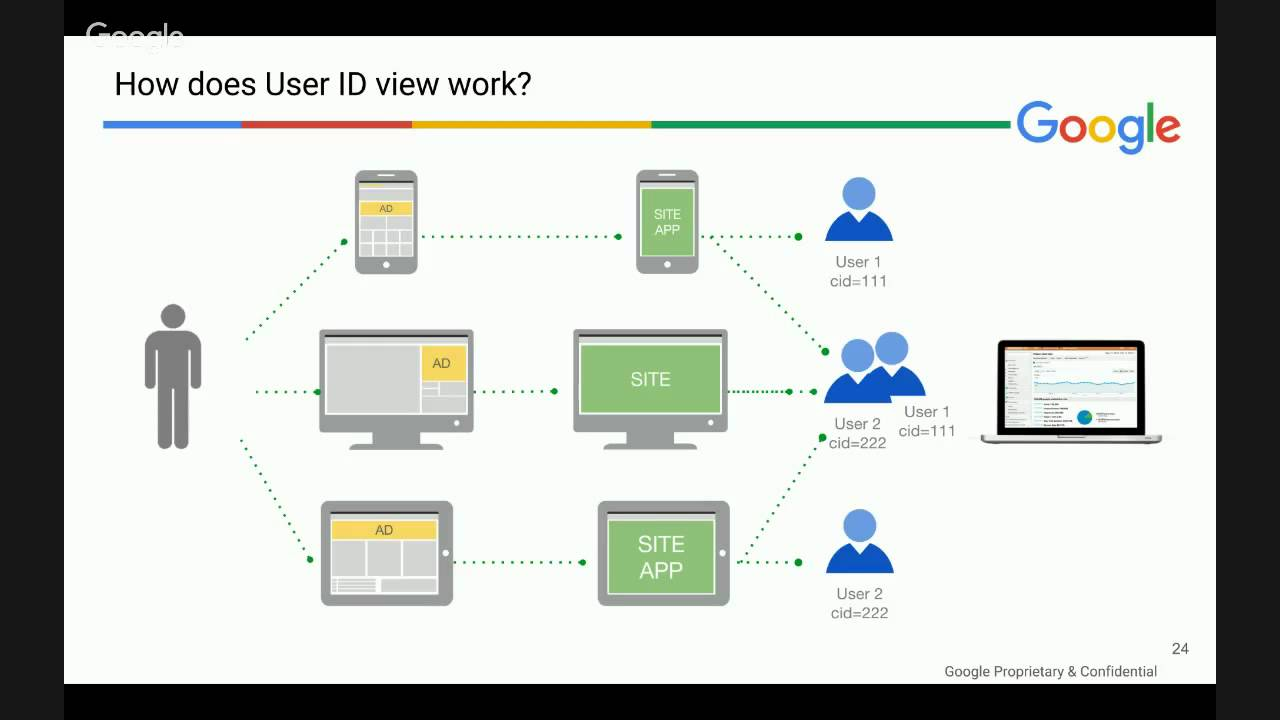
\includegraphics[width=0.7\textwidth]{graphics/userIdTracking.jpg}\\
			\tiny\url{https://https://tinyurl.com/z6u3b5e}
		\end{figure}	
		\item DEVICE-ID
			% Browser/Device Fingerprint
		\end{itemize}
		\end{frame}


	\subsection{Ultrasound Beacons (uBeacons)}		
		\begin{frame}\frametitle{Ultrasound Beacons (uBeacons) - Allgemein}
		\begin{itemize}
			\item Sind Grundlage aller Ultrasound-Tracking Produkte.
			\item Senden Schlagworte im Hochfrequenzbereich sog. "`tags"' in Form von kodierten Symbolen.
			\item Diese Signale können von den meisten kommerziellen Lautsprechern und Mikrophonen gesendet und empfangen werden.
			\item Die Signale sind nicht hörbar für den Menschen.
		\end{itemize}
		\end{frame}
		
		
		\begin{frame}\frametitle{Ultrasound Beacons (uBeacons) - Technische Details}
		\begin{itemize}
			\item Sendet in einem Spektrum von 18kHz bis 20kHz
			\item Aufteilung des Sendespektrums in  ca. 75Hz große Einheiten, woraus sich insgesamt ca. 26 Einheiten ergeben.
			\item Sendezeitraum für eine Einheit beträgt  ca. 4s.
			\item Die Enkodierung variiert dabei erheblich, da es keinen einheitlichen Standard und eine große Anzahl an unterschiedlichen Patenten gibt.
			\item Die gemessene Reichweite beträgt ungefähr 7m.
			\item Die Signale durchdringen keine physischen Hindernisse, wie Wände oder Türen.
		\end{itemize}
		\end{frame}
		
		\begin{frame}\frametitle{}
		\center\huge{XDT + uBeacon = uXDT}
		\end{frame}

	\subsection{Ultrasound Cross-Device Tracking (uXDT)}
		\begin{frame}\frametitle{Ultrasound Cross-Device Tracking (uXDT)}
		\begin{figure}[h]
			\centering
			\includegraphics[width=0.8\textwidth]{graphics/uXDT1.png}\\
			\tiny\url{https://tinyurl.com/zhflbjz}
		\end{figure}
		\end{frame}
		
		\begin{frame}\frametitle{Ultrasound Cross-Device Tracking (uXDT)}
		\begin{figure}[h]
			\centering
			\includegraphics[width=0.8\textwidth]{graphics/uXDT2.png}\\
			\tiny\url{https://tinyurl.com/zhflbjz}
		\end{figure}
		\end{frame}
		
		\begin{frame}\frametitle{Ultrasound Cross-Device Tracking (uXDT)}
		\begin{figure}[h]
			\centering
			\includegraphics[width=0.8\textwidth]{graphics/uXDT3.png}\\
			\tiny\url{https://tinyurl.com/zhflbjz}
		\end{figure}
		\end{frame}

\section{Tor Deanonymisierung}
	\subsection*{Tor Deanonymisierung}
		\begin{frame}\frametitle{Voraussetzungen}
			\begin{itemize}
				\item Tor-Nutzer
				\begin{itemize}
					\item Computer mit Lautsprecher und dem Tor-Browser.
					\item Smartphone in einem Umreis von 7m, welches eine uXDT-App verwendet.
				\end{itemize}
				\item Angreifer
			\end{itemize}
		\end{frame}
		
		\begin{frame}\frametitle{Ausgangsszenario}
		\begin{itemize}
			\item Ein Journalist(Jst) kooperiert mit dem Angreifer und will einen Whistleblower(Wb) identifizieren.
			\item Der Jst fordert den Wb auf seine Daten einem dafür eingerichteten Hidden-Service zu übergeben.
			\item Der Whistleblower startet den Tor-Browser und neben ihm liegt sein Smartphone. Das Ultraschall-Framework läuft im Hintergrund und horcht auf die Ultraschallsignale, die von den uBeacons gesendet werden. Er navigiert zum Hidden-Service und lädt die Daten hoch.
		\end{itemize}
		\end{frame}
		
		\begin{frame}\frametitle{Der Angriff}
		\begin{figure}[h]
			\centering
			\includegraphics[width=0.8\textwidth]{graphics/attac1.png}\\
			\tiny\url{https://tinyurl.com/zhflbjz}
		\end{figure}
		\end{frame}
		
		\begin{frame}\frametitle{Der Angriff}
		\begin{figure}[h]
			\centering
			\includegraphics[width=0.8\textwidth]{graphics/attac2.png}\\
			\tiny\url{https://tinyurl.com/zhflbjz}
		\end{figure}
		\end{frame}
		
%		\begin{frame}\frametitle{Ergebnis}
%		\begin{figure}[h]
%			\center
%			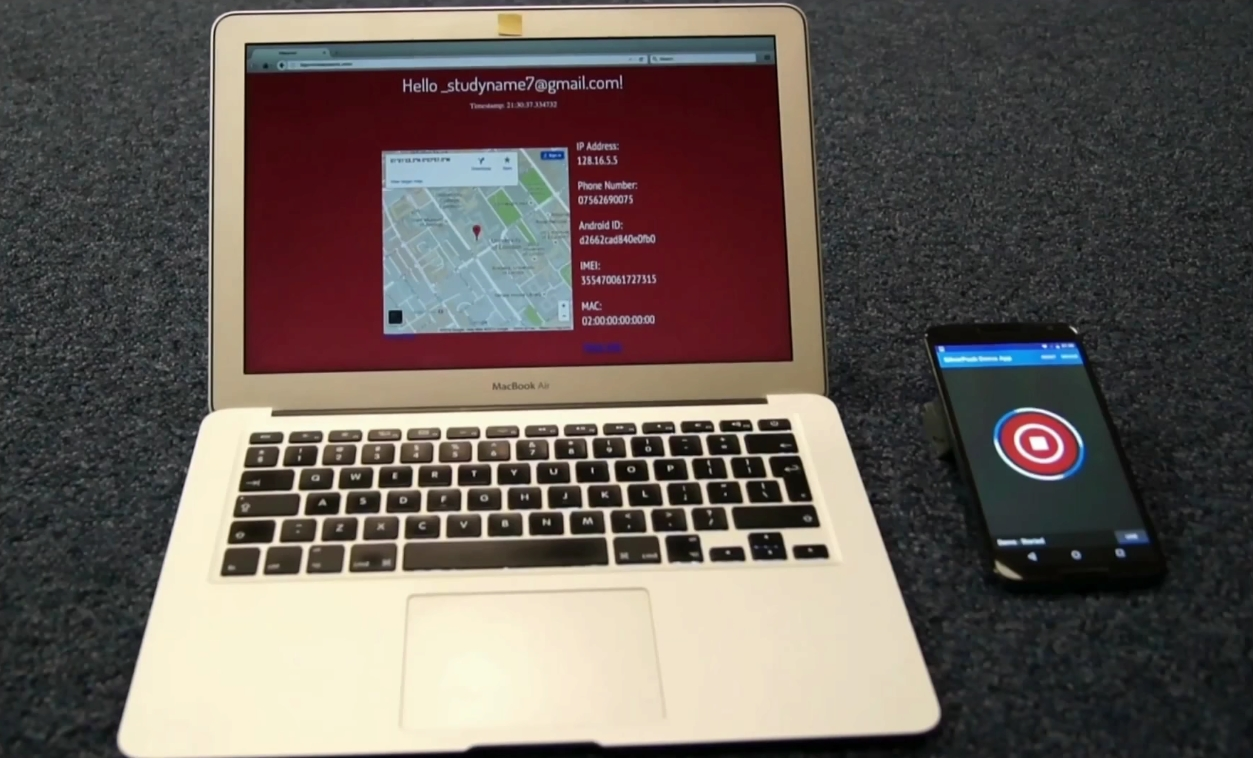
\includegraphics[width=0.8\textwidth]{graphics/Tor-Laptop.jpg}\\
%			\tiny\url{https://tinyurl.com/jgjqor4}
%		\end{figure}
%		\end{frame}
		
		\begin{frame}\frametitle{Ergebnis}		
		\begin{itemize}
			\item IP-Adresse
			\item Telefonnummer
			\item Android-ID
			\item Standort
			\item IMEI
			\item MAC
			\item GMail-Adresse
		\end{itemize}				
		% Grafik mit verändertem Ablauf
		\end{frame}

\section{Weitere Angriffsmöglichkeiten}
	\subsection*{Weitere Angriffsmöglichkeiten}
	
		\begin{frame}\frametitle{Weitere Angriffsmöglichkeiten}
		\begin{itemize}
			\item Tor de-anonymization Attack
			\item Profile corruption
			\item Information Leakage Attack
		\end{itemize}
		\end{frame}

\section{Schutzmechanismen}
	\subsection*{Wie kann man sich schützen?}
	
	\begin{frame}\frametitle{Schutz}
	\begin{itemize}
		\item Vasilios Mavroudis Team hat eine Browser-Extension entwickelt(SilverDog), welche die Ultraschallsignale herausfiltert.
		\item Im Zusammenhang mit der Extension kommt eine Android Permission zum Einsatz, die der App Zusatzberechtigungen einräumt, um auf die Audio-Einstellungen Einfluss zu nehmen.
		\item Eine Standartisierung muss gefordert werden
		\begin{itemize}
			\item uBeacon-Format
			\item Sicherheitseigenschaften
		\end{itemize}
		\item OS-Level API
		\begin{itemize}
			\item Bspw. Bluetooth für den Umgang und Entwicklung von uBeacons
			\item Erweitert die OS-Berechtigung im eine weitere API
		\end{itemize}
	\end{itemize} 
	\end{frame}
	
	\begin{frame}\frametitle{}
	\center\huge{Ende}
	\end{frame}

\section*{Quellen}\small
	\begin{frame}\frametitle{Quellen}
		\url{https://media.ccc.de/v/33c3-8336-talking_behind_your_back} \\
		\url{http://ubeacsec.org} \\
		\url{http://www.golem.de/news/anonymitaet-ultraschall-tracking-kann-tor-nutzer-deanonymisieren-1701-125434.html}
		\url{https://www.silverpush.co/\#!/} \\
		\url{https://www.blackhat.com/docs/eu-16/materials/eu-16-Mavroudis-Talking-Behind-Your-Back-Attacks-And-Countermeasures-Of-Ultrasonic-Cross-Device-Tracking.pdf}\\
	\end{frame}

\end{document}

